\apendice{Plan de Proyecto Software}
\label{apendice:plan_proyecto}

\section{Introducción}
\label{sec:plan_intro}

La planificación de un proyecto es una fase fundamental para su correcto desarrollo. En este apartado se comentará, por una parte, la planificación temporal del proyecto mediante los distintos \textit{sprints} que se han llevado a cabo, y por otra parte, se realizará un breve estudio sobre la viabilidad del proyecto.

En este proyecto se ha utilizado una metodología ágil basada en los principios de \textit{Scrum} \cite{trigas2012metodologia}. Para una correcta planificación, se optó por agrupar el trabajo en Épicas que contienen Sprints con objetivos temáticos, gestionando todas las tareas a través de un tablero en la plataforma \textbf{Jira} \cite{atlassian_jira}. Aunque las reuniones con los tutores eran periódicas para comentar dudas y avances, la estructura en sprints permitio un desarrollo iterativo y organizado.

\begin{figure}[H]
    \centering
    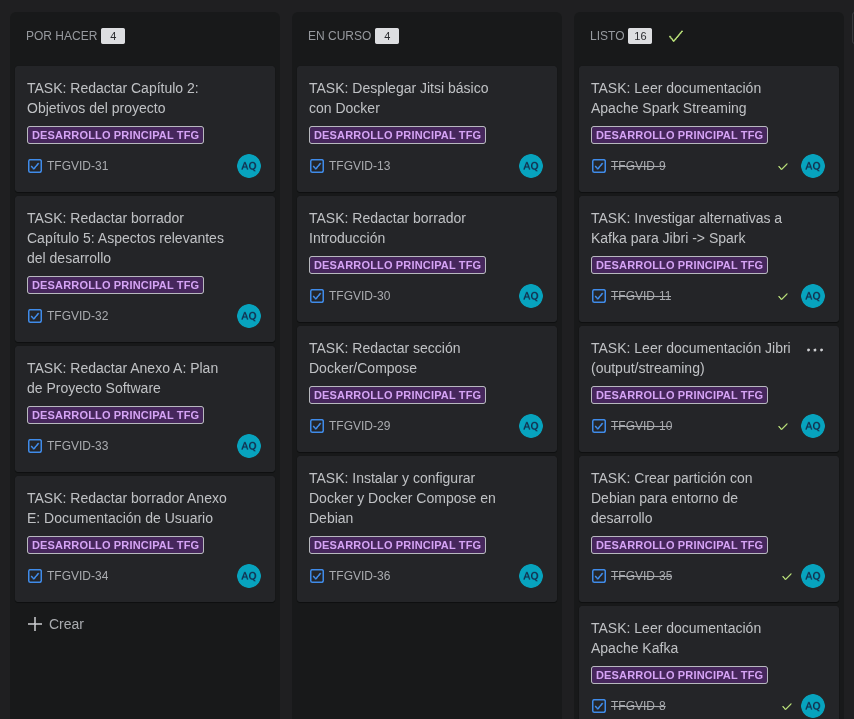
\includegraphics[width=\textwidth]{img/jira.png}
    \caption{Ejemplo del tablero Kanban utilizado en Jira para la gestión y seguimiento visual de las tareas del proyecto.}
    \label{fig:anexo_a_jira}
\end{figure}

\section{Planificación Temporal}
\label{sec:plan_temporal}
El desarrollo del proyecto se ha estructurado en Épicas que agrupan distintos \textit{sprints}, permitiendo un seguimiento claro de los grandes hitos del proyecto. A continuación, se detallan las fases y las tareas más relevantes de cada una, reflejando la evolución real del trabajo.

\begin{figure}[H]
    \centering
    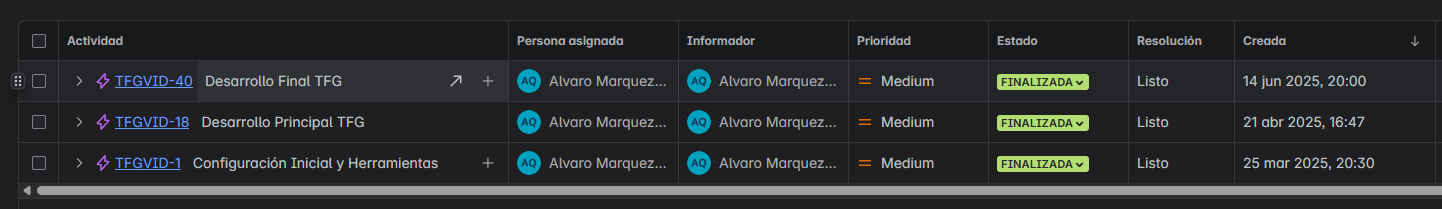
\includegraphics[width=\textwidth]{img/jira3.png}
    \caption{Ejemplo del épicas generadas durante el proyecto.}
    \label{fig:anexo_a_jira_epicas}
\end{figure}

\subsection{Épica 1: Investigación, Configuración y Desarrollo Inicial (Febrero 2025 - Abril 2025)}
\label{epic:1}
Esta primera épica abarcó desde el inicio del proyecto hasta la pausa de Semana Santa. El objetivo era establecer las bases teóricas y técnicas del TFG, asegurando que se contaba con el conocimiento y las herramientas adecuadas para comenzar el desarrollo.

\subsubsection{Sprint 1: Investigación y Configuración de Herramientas}
Este \textit{sprint} inicial fue de carácter exploratorio y de configuración. Se realizó una investigación exhaustiva de las tecnologías clave, se preparó el entorno de control de versiones y se configuraron las herramientas de gestión y documentación.

\begin{table}[H]
    \centering
    \begin{tabular}{|p{0.7\textwidth}|c|c|}
        \hline
        \rowcolor[HTML]{EFEFEF} 
        \textbf{Tareas (Jira ID)} & \textbf{Est.} & \textbf{Final} \\ \hline
        \rowcolor[HTML]{ECF4FF} 
        TASK: Investigar y seleccionar una plantilla \LaTeX{} para la UBU (TFGVID-2) & 2h & 2h \\
        \rowcolor[HTML]{EFEFEF} 
        TASK: Configurar repositorio GitHub con estructura inicial (doc/ y src/) (TFGVID-3) & 2h & 3h \\
        \rowcolor[HTML]{ECF4FF} 
        TASK: Configurar Overleaf y vincular con GitHub (si es posible) (TFGVID-4) & 2h & 2h \\
        \rowcolor[HTML]{EFEFEF} 
        TASK: Leer documentación Apache Kafka (TFGVID-8) & 16h & 20h \\
        \rowcolor[HTML]{ECF4FF} 
        TASK: Leer documentación Apache Spark Streaming (TFGVID-9) & 20h & 18h \\
        \rowcolor[HTML]{EFEFEF} 
        TASK: Leer documentación Jibri (output/streaming) (TFGVID-10) & 16h & 18h \\
        \rowcolor[HTML]{ECF4FF} 
        TASK: Investigar alternativas a Kafka para Jibri -> Spark (TFGVID-11) & 10h & 14h \\
        \hline
    \end{tabular}
    \caption{Tareas principales del Sprint 1.}
    \label{tab:sprint1}
\end{table}

La mayor dificultad durante este \textit{sprint} fue asimilar la gran cantidad de información sobre el ecosistema de tecnologías distribuidas, entendiendo cómo interactúan entre sí Kafka, Spark y Jitsi, así como sus complejas configuraciones.

\subsubsection{Sprint 2: Prototipado del Pipeline Base en Docker}
Con las herramientas ya investigadas, el objetivo de este \textit{sprint} fue crear un primer prototipo funcional de la infraestructura. Este \textit{sprint} se centró en la \textit{contenerización} de la aplicación y sus dependencias.

\begin{table}[H]
    \centering
    \begin{tabular}{|p{0.7\textwidth}|c|c|}
        \hline
        \rowcolor[HTML]{EFEFEF} 
        \textbf{Tareas (Jira ID)} & \textbf{Est.} & \textbf{Final} \\ \hline
        \rowcolor[HTML]{ECF4FF} 
        TASK: Crear Dockerfile básico para código Python (TFGVID-21) & 8h & 6h \\
        \rowcolor[HTML]{EFEFEF} 
        TASK: Construir y probar imagen Docker para script Python (TFGVID-22) & 16h & 18h \\
        \rowcolor[HTML]{ECF4FF} 
        TASK: Añadir Zookeeper a docker-compose.yml (TFGVID-27) & 8h & 10h \\
        \rowcolor[HTML]{EFEFEF} 
        TASK: Añadir Kafka a docker-compose.yml (TFGVID-28) & 4h & 7h \\
        \hline
    \end{tabular}
    \caption{Tareas principales del Sprint 2.}
    \label{tab:sprint2}
\end{table}

El principal desafío técnico fue la depuración de los primeros ficheros \texttt{Dockerfile} y \texttt{docker-compose.yml}, resolviendo errores relacionados con el contexto de construcción y la configuración de red entre contenedores.

\subsection{Épica 2: Despliegue, Depuración y Pivote de Infraestructura (Abril 2025 - Mayo 2025)}
\label{epic:2}
Esta segunda épica se centró en el despliegue del componente más complejo, Jitsi, y la resolución de los problemas de infraestructura que surgieron, lo que llevó a una decisión estratégica clave en el proyecto.

\subsubsection{Sprint 3 y 4: Despliegue de Jitsi, Bloqueo y Pivote Estratégico}
El objetivo inicial era desplegar una instancia de \texttt{docker-jitsi-meet} en Windows con WSL2. Esta fase se convirtió en un ciclo de depuración intensivo debido a errores de permisos en los volúmenes montados y fallos de autenticación de Jibri. Tras un intento infructuoso de implementar HTTPS, se tomó la decisión estratégica de migrar el entorno a Debian 12, donde, tras un nuevo ciclo de configuración, se logró un despliegue estable.

\begin{table}[H]
    \centering
    \resizebox{\textwidth}{!}{
    \begin{tabular}{|p{0.8\textwidth}|c|c|}
        \hline
        \rowcolor[HTML]{EFEFEF} 
        \textbf{Tareas de los Sprints 3 y 4 (Jira ID)} & \textbf{Est.} & \textbf{Final} \\ \hline
        \rowcolor[HTML]{ECF4FF} 
        TASK: Desplegar Jitsi básico con Docker (local) (TFGVID-13) & 20h & 30h \\
        \rowcolor[HTML]{EFEFEF} 
        TASK: (Cancelada) Implementar HTTPS en Jitsi local & 6h & 6h \\
        \rowcolor[HTML]{ECF4FF} 
        TASK: Instalar y configurar Docker y Docker Compose en Debian (TFGVID-26) & 20h & 24h \\
        \rowcolor[HTML]{EFEFEF} 
        TASK: Configurar data-root de Docker para gestión de disco & 8h & 7h \\
        \rowcolor[HTML]{ECF4FF} 
        TASK: Solucionar error de montaje del contenedor web de Jitsi & 8h & 8h \\
        \hline
    \end{tabular}
    }
    \caption{Tareas principales de los Sprints 3 y 4.}
    \label{tab:sprint3_4}
\end{table}

\subsection{Épica 3: Finalización del Proyecto (Mediados de Mayo 2025 en adelante)}
\label{epic:3}
Esta épica final engloba todas las tareas restantes para la conclusión del proyecto, divididas en una fase final de implementación técnica y una fase de documentación y entrega.
\begin{table}[H]
    \centering
    \resizebox{\textwidth}{!}{
    \begin{tabular}{|l|p{0.7\textwidth}|c|c|}
        \hline
        \rowcolor[HTML]{EFEFEF} 
        \textbf{Fase} & \textbf{Tareas} & \textbf{Est.} & \textbf{Final} \\ \hline
        \rowcolor[HTML]{ECF4FF} 
        \multirow{7}{*}{\parbox{2cm}{\textbf{Implementación Técnica}}} & TASK: Preparar entorno limpio para el despliegue de Jitsi & 2h & 3h \\
        \rowcolor[HTML]{EFEFEF}
         & TASK: Implementar HTTPS en Jitsi con Certificados Let's Encrypt & 16h & 14h \\
        \rowcolor[HTML]{ECF4FF} 
         & TASK: Validar la grabación de vídeo con Jibri & 16h & 24h \\
        \rowcolor[HTML]{EFEFEF} 
         & TASK: Configurar el entorno de procesamiento con Spark & 18h & 20h \\
        \rowcolor[HTML]{ECF4FF} 
         & TASK: Desarrollar el script de procesamiento de vídeo (Prueba de Concepto) & 8h & 7h \\
        \rowcolor[HTML]{EFEFEF} 
         & TASK: Integrar y probar el pipeline completo (Jitsi -> Spark) & 20h & 16h \\
         \rowcolor[HTML]{ECF4FF}
         & TASK: Definir y documentar el formato de salida de los resultados & 4h & 6h \\
         \hline
        \rowcolor[HTML]{EFEFEF} 
        \multirow{7}{*}{\parbox{2cm}{\textbf{Documentación y Entrega}}} & TASK: Documentar el despliegue y la depuración de Jitsi & 6h & 6h \\
        \rowcolor[HTML]{ECF4FF} 
         & TASK: Documentar la implementación del pipeline de Spark & 6h & 6h \\
        \rowcolor[HTML]{EFEFEF} 
         & TASK: Finalizar el diseño de la arquitectura y el diagrama de flujo & 8h & 6h \\
        \rowcolor[HTML]{ECF4FF} 
         & TASK: Redactar la versión final del Manual de Usuario & 6h & 6h \\
        \rowcolor[HTML]{EFEFEF} 
         & TASK: Escribir las conclusiones y realizar la revisión final & 6h & 6h \\
        \rowcolor[HTML]{ECF4FF} 
         & TASK: Preparar el repositorio de GitHub para la entrega & 4h & 6h \\
        \rowcolor[HTML]{EFEFEF}
         & TASK: Realizar Anexo de Sostenibilidad Curricular & 4h & 6h \\
        \hline
    \end{tabular}
    }
    \caption{Tareas del Epic 3: Finalización del Proyecto.}
    \label{tab:epic3}
\end{table}

\section{Estudio de viabilidad}
\label{sec:plan_viabilidad}
En este apartado se va a comentar la viabilidad del proyecto. Por una parte, se redactará la \emph{viabilidad económica}, que hará referencia al coste que supondría el desarrollo del proyecto si se realizara en un entorno empresarial, y por otra parte, se detallará la \emph{viabilidad legal} de las herramientas y librerías utilizadas.

\subsection{Viabilidad económica}
En este apartado se presentan unos cálculos económicos teóricos para desarrollar el proyecto. Para realizar el cálculo, se han dividido los gastos en:
\begin{enumerate}
    \item \textbf{Coste de personal}: en la tabla \ref{tablaA1} se encuentra una estimación del coste que supondría contratar a un ingeniero de software durante la duración del TFG (aproximadamente 6 meses).
    \item \textbf{Coste \textit{hardware}}: la tabla \ref{tablaA2} contiene la inversión en el \textit{hardware} necesario para el desarrollo.
    \item \textbf{Coste de servicios}: la tabla \ref{tablaA3} detalla los servicios externos utilizados.
\end{enumerate}
Finalmente, en la tabla \ref{tablaA4} se puede observar un cálculo final del coste teórico del proyecto.

\begin{table}[H]
    \centering
    \begin{tabular}{lc}
        \hline
        \rowcolor[HTML]{EFEFEF} 
        \multicolumn{1}{c}{\cellcolor[HTML]{EFEFEF}\textbf{Concepto}} & \textbf{Coste (€)} \\ \hline
        \rowcolor[HTML]{ECF4FF} 
        Salario mensual bruto (Ingeniero de Software Jr.) \cite{salariales_tic} & 2.100,00 \\
        \rowcolor[HTML]{EFEFEF} 
        Seguridad Social a cargo de la empresa (aprox. 31\%) & 651,00 \\ \hline
        \rowcolor[HTML]{ECF4FF} 
        \textbf{Coste mensual por empleado} & \textbf{2.751,00} \\ \hline
        \rowcolor[HTML]{EFEFEF} 
        \textbf{Total 6 meses (1 empleado)} & \textbf{16.506,00} \\ \hline
    \end{tabular}
    \caption{Costes de personal.}
    \label{tablaA1}
\end{table}

\begin{table}[H]
    \centering
    \begin{tabular}{lcc}
        \hline
        \rowcolor[HTML]{EFEFEF} 
        \multicolumn{1}{c}{\cellcolor[HTML]{EFEFEF}\textbf{Concepto}} & \textbf{Coste (€)} & \textbf{Coste amortizado (4 años)} \\ \hline
        \rowcolor[HTML]{ECF4FF} 
        Ordenador de desarrollo & 1.200,00 & 150,00 \\
        \rowcolor[HTML]{EFEFEF} 
        Servidor/Host para despliegue & 2.000,00 & 250,00 \\ \hline
        \rowcolor[HTML]{ECF4FF} 
        \textbf{Total} & \textbf{3.200,00} & \textbf{400,00} \\ \hline
    \end{tabular}
    \caption{Costes de \textit{hardware}.}
    \label{tablaA2}
\end{table}

\begin{table}[H]
    \centering
    \begin{tabular}{lc}
        \hline
        \rowcolor[HTML]{EFEFEF} 
        \multicolumn{1}{c}{\cellcolor[HTML]{EFEFEF}\textbf{Concepto}} & \textbf{Coste mensual (€)} \\ \hline
        \rowcolor[HTML]{ECF4FF} 
        Conexión a Internet de alta velocidad & 50,00 \\
        \rowcolor[HTML]{EFEFEF} 
        Dominio y servicio DuckDNS & 0,00 (Gratuito) \\ \hline
        \rowcolor[HTML]{ECF4FF} 
        \textbf{Total (por 6 meses)} & \textbf{300,00} \\ \hline
    \end{tabular}
    \caption{Costes de servicios.}
    \label{tablaA3}
\end{table}

\begin{table}[H]
    \centering
    \begin{tabular}{lc}
        \hline
        \rowcolor[HTML]{EFEFEF} 
        \multicolumn{1}{c}{\cellcolor[HTML]{EFEFEF}\textbf{Concepto}} & \textbf{Coste (€)} \\ \hline
        \rowcolor[HTML]{ECF4FF} 
        Personal (6 meses) & 16.506,00 \\
        \rowcolor[HTML]{EFEFEF} 
        \textit{Hardware} (amortizado 6 meses) & 400,00 \\
        \rowcolor[HTML]{ECF4FF} 
        Servicios (6 meses) & 300,00 \\ \hline
        \rowcolor[HTML]{EFEFEF} 
        \textbf{Coste total estimado del proyecto} & \textbf{17.206,00} \\ \hline
    \end{tabular}
    \caption{Coste total teórico del proyecto.}
    \label{tablaA4}
\end{table}

\subsection{Viabilidad legal}
En este subapartado se exponen las distintas licencias que tienen las herramientas y librerías utilizadas, así como la licencia final con la que cuenta este proyecto. En la tabla \ref{tablaA5} se muestran las tecnologías utilizadas y su correspondiente licencia.

\begin{table}[H]
    \centering
    \begin{tabular}{lc}
        \hline
        \rowcolor[HTML]{EFEFEF} 
        \textbf{Librería/Herramienta} & \textbf{Licencia} \\ \hline
        \rowcolor[HTML]{ECF4FF} 
        \textit{Debian 12} & GPL y otras FOSS \\
        \rowcolor[HTML]{EFEFEF} 
        \textit{Docker} & Apache 2.0 \\
        \rowcolor[HTML]{ECF4FF} 
        \textit{Apache Kafka} & Apache 2.0 \\
        \rowcolor[HTML]{EFEFEF} 
        \textit{Apache Spark} & Apache 2.0 \\
        \rowcolor[HTML]{ECF4FF} 
        \textit{Jitsi Meet} & Apache 2.0 \\
        \rowcolor[HTML]{EFEFEF} 
        \textit{Python} & Python Software Foundation License \\
        \rowcolor[HTML]{ECF4FF} 
        \textit{OpenCV-Python} & GNU v3.0 License \\
        \rowcolor[HTML]{EFEFEF} 
        \textit{NumPy} & BSD 3-Clause \\
        \hline
    \end{tabular}
    \caption{Tabla con las licencias de las herramientas utilizadas.}
    \label{tablaA5}
\end{table}

La licencia final escogida para el código fuente de este proyecto ha sido \textbf{GNU v3.0 License}, ya que es una licencia de software libre muy permisiva que permite su reutilización en prácticamente cualquier escenario, incluyendo proyectos comerciales, sin imponer grandes restricciones.

\subsubsection{\textit{Copyright} de terceros}
Este proyecto se ha construido sobre el trabajo de comunidades y organizaciones de código abierto. A continuación, se detallan los principales titulares de derechos de las tecnologías utilizadas:
\begin{itemize}
	\item \textbf{Apache 2.0}:
	    \begin{itemize}
	        \item \textit{Apache Kafka} - The Apache Software Foundation
	        \item \textit{Apache Spark} - The Apache Software Foundation
	        \item \textit{Docker} - Docker, Inc.
	        \item \textit{Jitsi Meet} - 8x8, Inc.
	    \end{itemize}
	\item \textbf{BSD y GNU v3.0}:
	    \begin{itemize}
	        \item \textit{NumPy} - The NumPy community
	        \item \textit{OpenCV} - OpenCV team
	    \end{itemize}
    \item \textbf{PSF}:
	    \begin{itemize}
	        \item \textit{Python} - Python Software Foundation
	    \end{itemize}
\end{itemize}